\documentclass[a4paper,10pt]{article}
\usepackage[utf8]{inputenc}
\usepackage{fullpage}
\usepackage{graphicx}
\usepackage{subcaption}
\usepackage[authoryear]{natbib}
\usepackage{tikz}
\usetikzlibrary{spy}

%opening
\title{GIS-based UAV/Lidar DSM fusion for water flow modeling}
\author{Anna Petrasova}

\begin{document}
\maketitle
\section*{Introduction}
The fusion of digital elevation models has become an important technique
as the spectrum of sensors, DEM spatial and temporal resolutions and extents grows.
Common use cases include deriving more accurate DEM from multiple sources with different geometric
and accuracy characteristics, updating older DEMs with newer measurements, or locally enhancing
lower resolution DEM with higher resolution information.
Several authors have proposed different fusion methods of large scale DEMs 
(such as SRTM, GDEM, ASTER)
including frequency domain filtering \citep{Karkee2008}, or weighted averaging \citep{Tran2014, Papasaika2011},
where weights can be derived differently, for example, based on DEM's accuracy assessment.

Our use case is to fuse lidar data with high resolution UAS-derived digital surface model
for the purpose of modeling overland water flow. Although lidar surveys deliver data
in increasingly high resolution, the microtopography is often not captured
or the repeating surveys necessary to study changes are not economically feasible.
By combining best of both types of data -- large extent and bare ground information with
up-to-date and high resolution information -- we can model water flow and sediment transport more reliably.

I will review several raster and vector based fusion techniques which can be used for situations when
we want to replace certain areas in one DEM by a different DEM, which is different case than
most literature discusses.


\section*{Methods}

\subsection*{DEM differences}
Analyzing and possibly correcting differences is important for a successful fusion of DEMs.
We analyzed the differences between lidar and UAS in previous class homeworks
and as we learned the lidar was mostly higher (around 10 cm) than the UAV data (and the GCPs),
however the differences between lidar and UAV DSM, and among UAV DSMs, have more complex and unpredictable 
pattern. Although the absolute differences are mostly around 10 cm, they can reach 20 cm which 
can cause noticeable discontinuities.

Since we don't have any reference surface we would know is accurate, we can use the lidar DEM as
a reference and modify the UAV DSMs based on it. One approach is to use linear regression
on the whole surface and modify it to optimally match the reference.
This might not be enough if there are significant local distortions.
For this purpose we can derive a smoothed difference and apply it on the UAV DSM.
It can be derived for example using r.neighbors median function with large window size on a difference raster.
This however may take a long time to compute if we run it with the same high resolution,
because the moving window analysis is computed for each pixel.
I used a faster alternative where I compute the median for a window of desired size 
for points in a regular grid and then interpolate those values.
In any case, the difference raster should be (prior to computation) free of high values we know are not part of the distorion,
but are rather caused by changes in vegetation. These can be filtered using simple raster algebra.

Such smoothed difference can be then subtracted from (or added to) the UAV DSM and obtain the corrected one,
see Figure \ref{fig:distortion}.

\begin{figure}
	\centering
        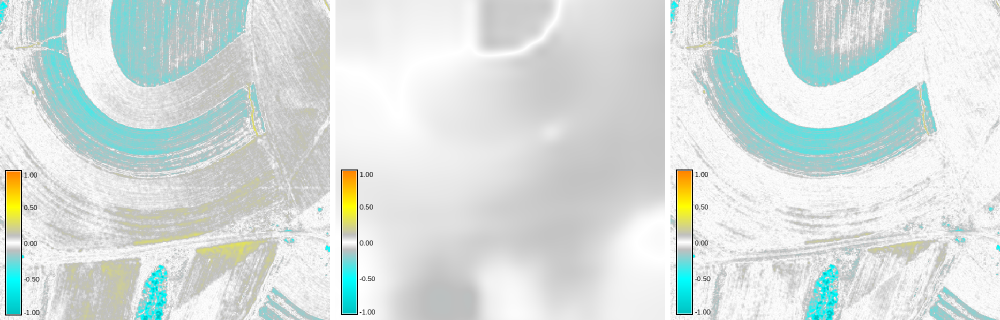
\includegraphics[width=\textwidth]{img/distortion.png}
	\caption{Original, smoothed and corrected difference between March UAV DSM and lidar DEM}
	\label{fig:distortion}
\end{figure}

\subsection*{GIS-based fusion techniques}
The discussed fusion techniques include:

\paragraph*{Weighted average smoothing along edges}
This method is suitable when we have two or more rasters which need to be patched together
and the values at the edges are close enough. We compute distance from the edge and normalize it,
and combine 2 rasters using raster algebra and the following formula:

$$z_F = d \cdot z_{UAV} + (1 - d) \cdot z_{lidar}\quad d\in \langle0, 1\rangle$$


\begin{figure}[bc]
	\centering
	\begin{subfigure}[b]{0.33\textwidth}
 		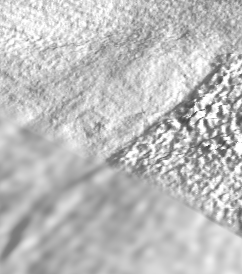
\includegraphics[width=\textwidth]{img/sm1}
	\end{subfigure}\hfill%
	%
	\begin{subfigure}[b]{0.33\textwidth}
		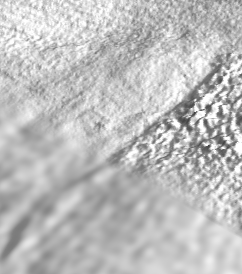
\includegraphics[width=\textwidth]{img/sm2}
	\end{subfigure}\hfill%
	\begin{subfigure}[b]{0.33\textwidth}
 		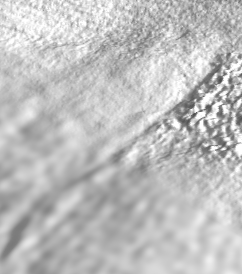
\includegraphics[width=\textwidth]{img/sm3}
	\end{subfigure}\hfill%
	\caption{Smoothing along edge: 5 m, 10 m, 30 m}
	\label{fig:smoothing}
\end{figure}

With different choice of distance threshold, the effect of smoothing changes,
see Figure \ref{fig:smoothing}. I implemented 
this fusion in a script r.patch.smooth which is available through g.extension on Linux and Mac:

{\small
\begin{verbatim}
g.extension r.patch.smooth url="https://github.com/petrasovaa/r.patch.smooth"
\end{verbatim}}


\paragraph*{Patching point clouds and interpolation}
When we have the original point clouds we can combine them using mask to distinguish
area where each point cloud should be applicable. This can be done with 
the recent additions in v.in.lidar (option mask and flag -i).
Next step is patching and interpolating the point cloud.
However, there could be visible edge depending on how well the point clouds match at the transition zone.
For this reason, we may need to buffer the edge and create
a narrow gap to be filled by the interpolation, see Figure \ref{fig:points}.

\begin{figure}
	\centering
        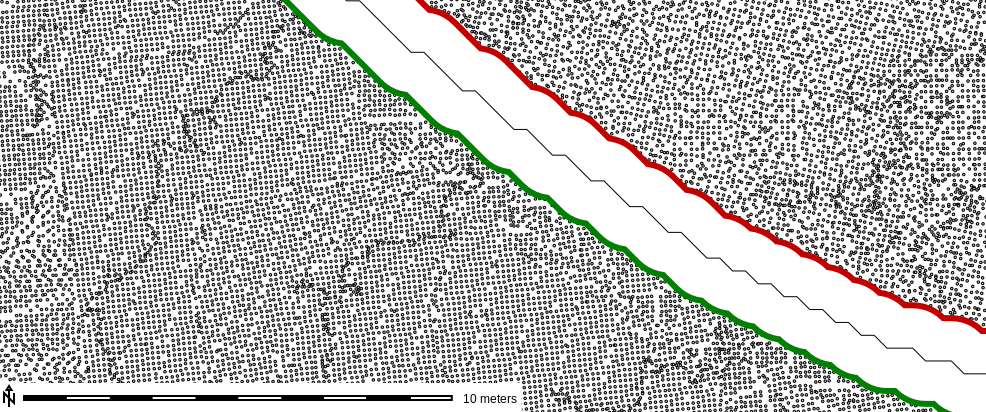
\includegraphics[width=0.9\textwidth]{img/points.png}
	\caption{Patched point cloud with gap}
	\label{fig:points}
\end{figure}

\paragraph*{Resampling DEMs and re-interpolation}
Another vector-based method is suitable typically when we don't have original
point clouds but we have raster data. We first patch the rasters in a simple way,
use r.random to randomly sample the digital elevation models and then patch them
and continue by re-interpolating them.
It is crucial to sample by sufficient number of points to avoid missing features
(I~used 2 points per cell).
As in the previous case, it is possible to leave a narrow gap of NULL
on the edge of the rasters when patching; this will result in no sampling points
and interpolation takes care of the gap.



\section*{Applications}

I will show the performance and use cases of the described
methods on 2 examples. One is the fusion of UAV data from different times
and the other one is fusing lidar data with data from scanning using 
Tangible Landscape.

\subsection*{Mid Pines March and June fusion}
For testing the fusion workflows, I decided to fuse
March and June DSMs to create a bare earth surface. 
March and June DSMs have the crops planted in the opposite bands
and therefore we can recover the bare earth information (Figure \ref{fig:march}).

 \begin{figure}
	\centering
	\begin{subfigure}[b]{0.49\textwidth}
 		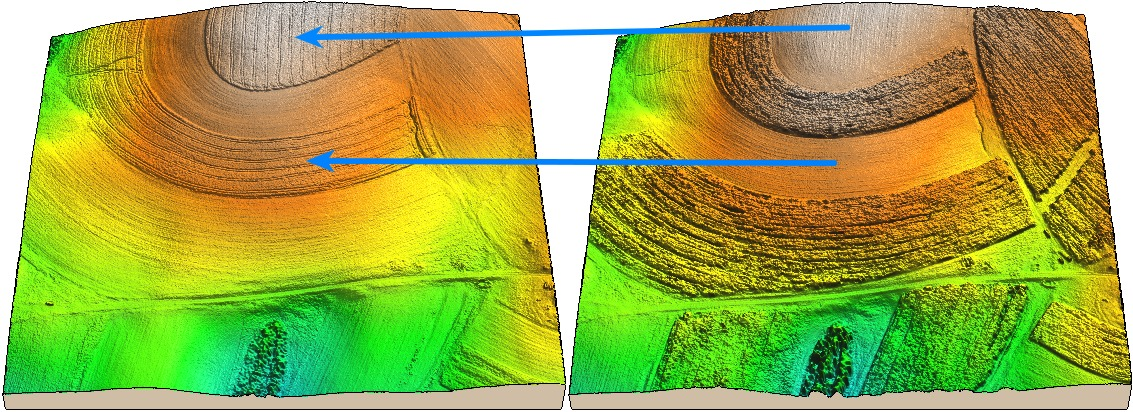
\includegraphics[width=\textwidth]{img/march}
 		\caption{\label{fig:march}}
	\end{subfigure}\hfill%
	\begin{subfigure}[b]{0.25\textwidth}
 		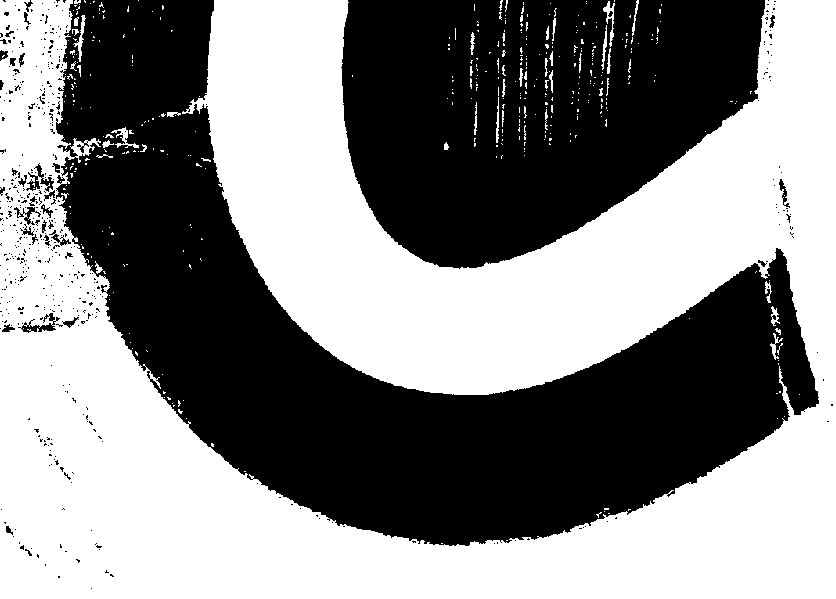
\includegraphics[width=\textwidth]{img/mask}
 		\caption{}
	\end{subfigure}\hfill%
	\begin{subfigure}[b]{0.25\textwidth}
 		
\includegraphics[width=\textwidth]{img/mask_sm}
 		\caption{}
	\end{subfigure}\hfill%
	\caption{(a) March and June DSMs, (b) mask created with r.series min\_raster and (c) the same after filtering}
	\label{fig:march_mask}
\end{figure}

For this particular case, the weighted average fusion was not an option
because it would create an artificial feature in the transition zone
since both DSMs are very different there due to crop rotation.
Therefore I used the other methods discussed.

A simplest method of fusion in this special case is using r.series with method minimum
because I am trying to get bare earth. Because this method works pixel by pixel,
it can create some artificial discontinuities (see Figure \ref{fig:res}).
However, by applying r.series
with method min\_raster
we can obtain a raster representing a mask necessary for the fusion process.
Filtering the mask with mode operator
makes the shape of the mask more compact (Figure \ref{fig:march_mask}).

Then we can apply the methods described in the previous section.
For both vector-based workflows I had to buffer the edge to create a gap with no points,
1 m on both sides, otherwise the resulting interpolated DSM had an artificial bump
which we know is not there because it is not visible
on the late October DSM (the one with no crops).
I ran r.sim.water on the fused surfaces and as we can see in Figure
\ref{fig:res}, both vector-based methods perform very similarly. The minimum 
raster method produces visible bumps on the edges, but considering
it is a very simple method, the results are quite good.

 \begin{figure}
	\centering
	\begin{subfigure}[b]{0.74\textwidth}
 		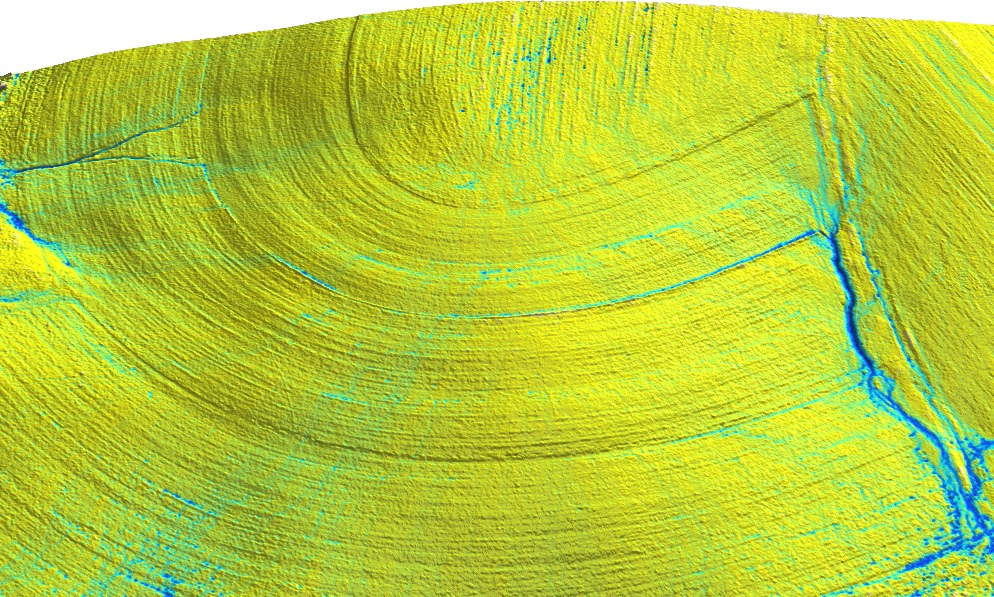
\includegraphics[width=\textwidth]{img/min}
 		\caption{\label{fig:res_1}}
	\end{subfigure}\hfill%
	\begin{subfigure}[b]{0.74\textwidth}
 		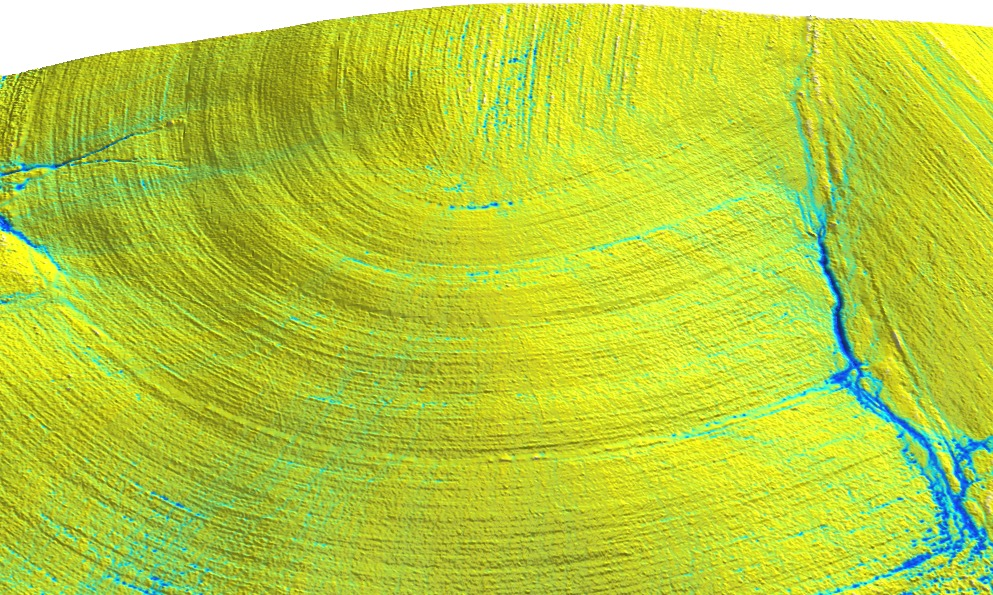
\includegraphics[width=\textwidth]{img/mask_interp}
 		\caption{}
	\end{subfigure}\hfill%
	\begin{subfigure}[b]{0.74\textwidth}
 		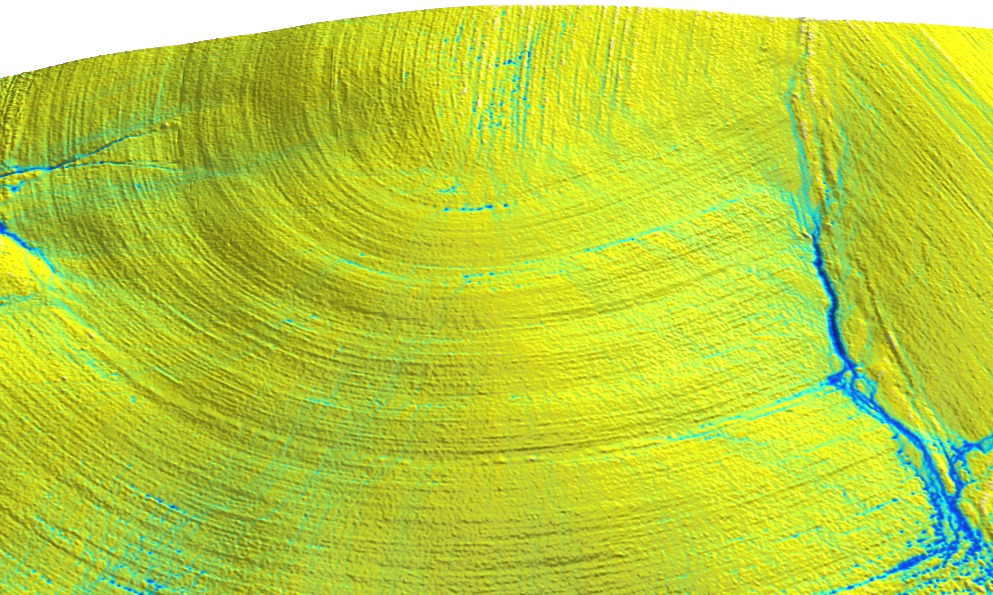
\includegraphics[width=\textwidth]{img/sampling}
 		\caption{}
	\end{subfigure}\hfill%
	\caption{Water flow simulation on surfaces derived with 
	(a) r.series minimum, (b) patching point clouds and interpolation
	and (c) resampling DEMs and re-interpolation}
	\label{fig:res}
\end{figure}


\subsection*{Tangible Landscape}
When using Tangible Landscape, the scale of the interaction is always a difficult decision.
Taking water flow modeling example, we need to interact at fine scale and thus on a model
with small extent, but 
our changes then both depend and have influence on larger area outside of the physical model.
As shown in \cite[Chapter 9 Fire]{Petrasova2015}, it is easy to patch smaller extent of interaction
into larger modeling extent if we don't need smooth transition. In case of water flow,
the smoothness of transition is very important. I apply here the 
weighted difference as best method from the ones discussed, since it is very fast.

I built a physical model of a small part of Mid Pineas area based on the lidar data in scale 1 : 420 with
4 times vertical exaggeration by projecting contours and color-coded difference. In Figure 
\ref{fig:model_ortho_all} we can see projected orthophoto and watershed boundaries.
I ran r.sim.water simulation over the entire area of that watershed with the fused
scan of the model into lidar DEM. The resulting water depth matches the location of the gully, which shows
I modeled the shape of the valley quite accurately based on the contours and color-coded difference.
The fused surface is visible in Figure \ref{fig:fusion}, we can still see
the transition and also the rough surface from scanner, but that's something
which could be improved by different parameters of interpolation of the scan.

I tried a scenario when I moved the stream to the east outside of the field
and created small checkdams to capture and slow down the rainfall water (Figure \ref{fig:diff2}).
As visible, to move the stream to the east, the changes in volume
were quite small, under 30 cm, as they don't show up in the cut and fill figure.





\begin{figure}
\centering
 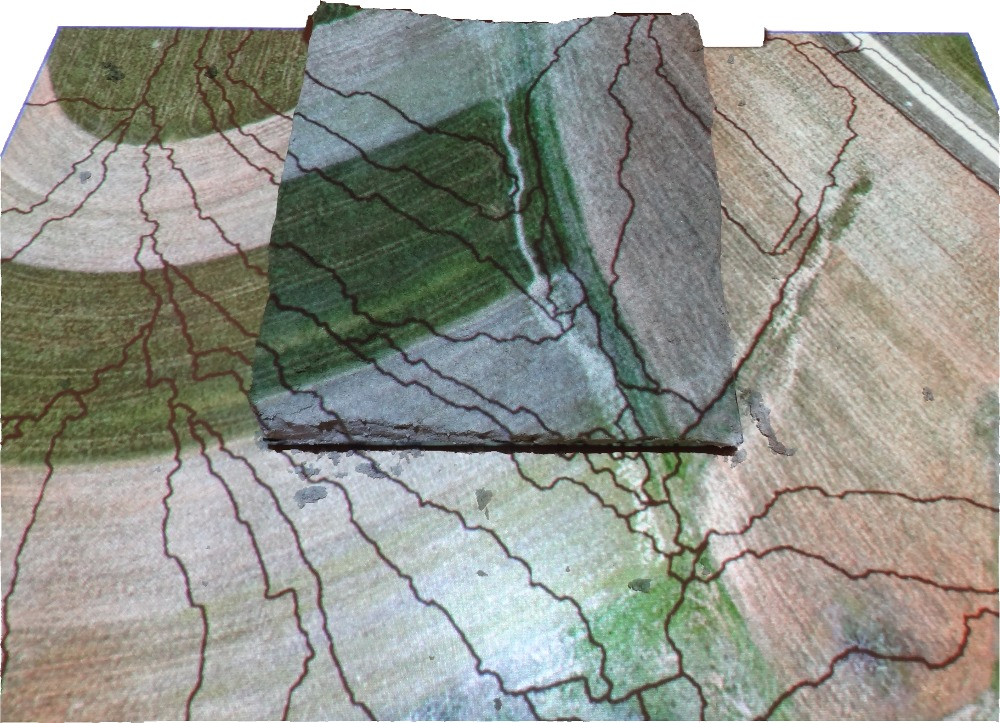
\includegraphics[width=0.7\textwidth]{img/model_ortho_all}
 \caption{Model with projected ortho and basins}
 \label{fig:model_ortho_all}
\end{figure}
\begin{figure}
\centering
 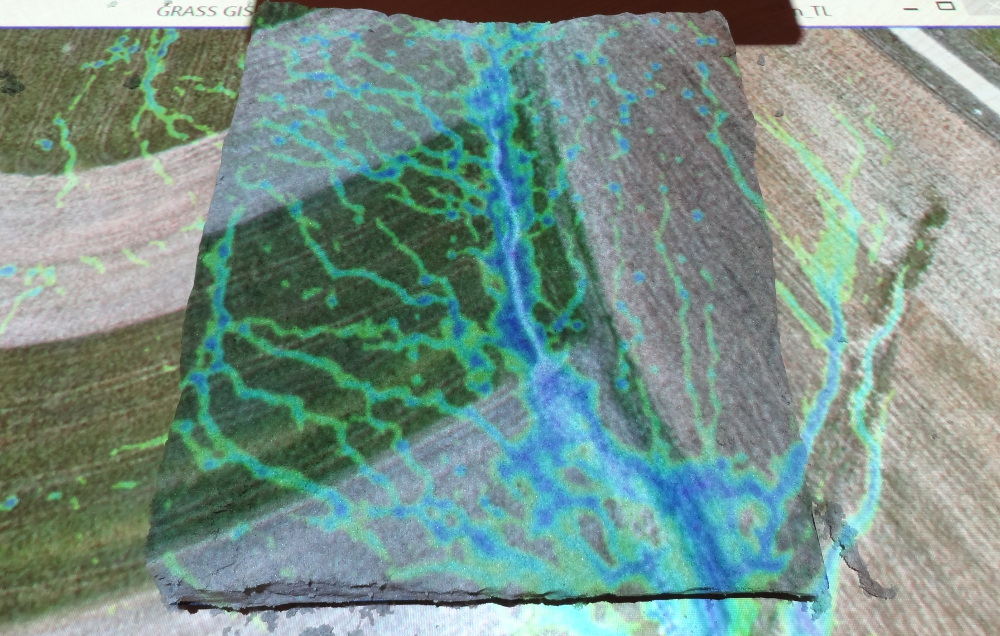
\includegraphics[width=0.7\textwidth]{img/flow1_detail}
 \caption{Model with projected r.sim.water simulation}
  \label{fig:flow1_detail}
\end{figure}

\begin{figure}
\centering
 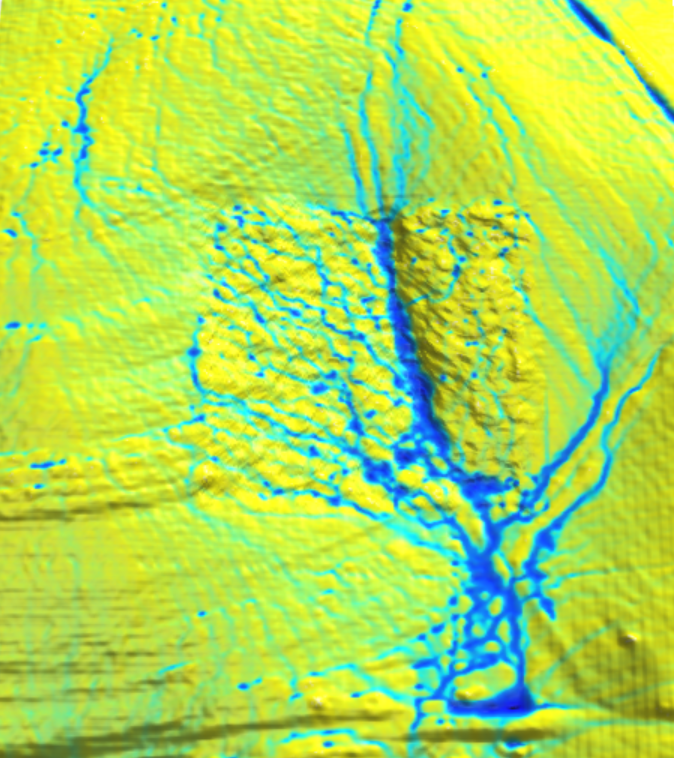
\includegraphics[width=0.5\textwidth]{img/fusion}
 \caption{Fusion of lidar data and scanned data 3 times exaggerated}
  \label{fig:fusion}
\end{figure}


\begin{figure}
	\centering
	\begin{subfigure}[b]{0.499\textwidth}
 		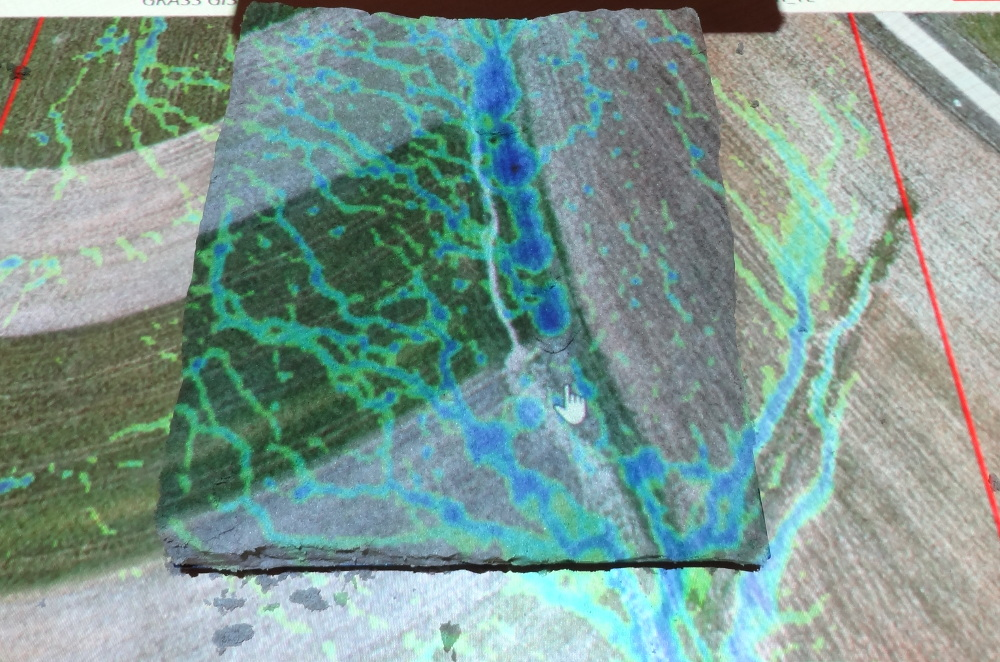
\includegraphics[width=\textwidth]{img/flow2}
 		\caption{}
	\end{subfigure}\hfill%
	\begin{subfigure}[b]{0.499\textwidth}
 		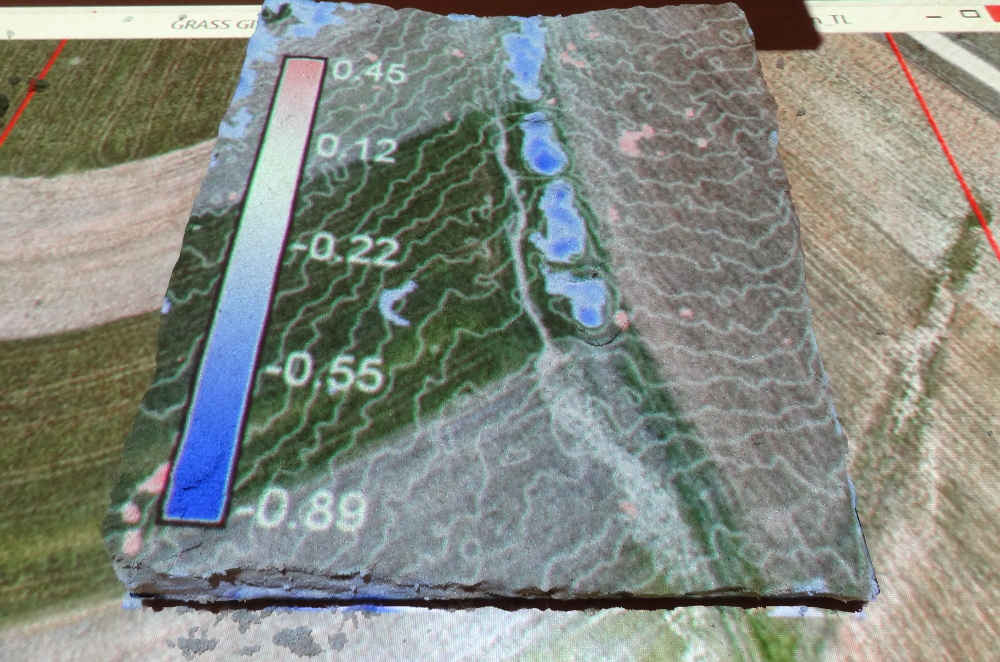
\includegraphics[width=\textwidth]{img/diff2}
 		\caption{}
	\end{subfigure}\hfill%
	\caption{(a) checkdam scenario  and (b) necessary cut and fill (highlighted 
	changes greater than 30 cm)}
	\label{fig:diff2}
\end{figure}

\section*{Conclusion}
I explored different  DEM and DSM fusion techniques in the context of overland water flow 
modeling on high resolution surfaces and demonstrated their usage on 2 applications.
Selecting the appropriate technique depends on the input data available (raster or vector)
and time available for computation, which can be restricted 
(for example for real-time scanning application).
\bibliographystyle{plainnat}
\bibliography{references} 
\end{document}
